\chapter{Two-Loop Holomorphy and Non-Renormalization Theorems\label{ch:2looptheorems}}

\begin{flushright}
\small

{\color{chapterpaperrule}\rule{\textwidth}{0.5pt}}

\textit{This chapter is based on:}\\[0.5em]
L.~C.~Bresciani and N.~Selimovic,\\[0pt]
``Two-Loop Holomorphy and Non-Renormalization Theorems in Effective Field Theories,''\\[0pt]
(to be published).

{\color{chapterpaperrule}\rule{\textwidth}{0.5pt}}
\end{flushright}

\lb{Insert incipit and outline.}

%%%%%%%%%%%%%%%%%%%%%%%%%%%%%%%%%%
\begin{figure}[t]
    \centering
    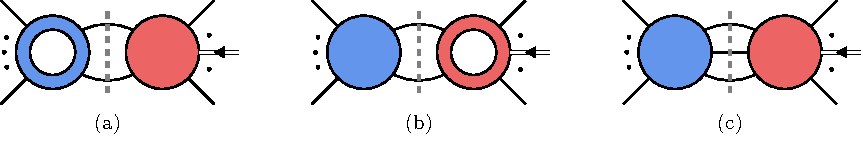
\includegraphics[page=1]{images/cuts.pdf}
    \caption{Unitarity cuts relevant for the extraction of anomalous dimensions from two-loop form factors. Higher-dimensional operator insertions are indicated by red blobs. The blobs with a hole denote one-loop form factors or amplitudes.}
    \label{fig:cuts}
\end{figure}
%%%%%%%%%%%%%%%%%%%%%%%%%%%%%%%%%%

\section{Scheme-Independent Zeros}

We first collect the two-loop zeros that follow from tree-level data alone and are therefore scheme independent. 
The length selection rule of Ref.~\cite{Bern:2019wie} already forbids a large class of entries: the form-factor side of any cut of $\mathcal O_j$ appearing in Eq.~\eqref{eq:master} needs at least $\ell_j$ legs, so an operator $\mathcal O_j$ cannot renormalize a shorter operator $\mathcal O_i$ at two loops when $\ell_j - \ell_i \ge 2$, since no such diagram can avoid a scaleless integral. Thus, $\gamma^{(2)}_{ij} = 0$ if $\ell_i < \ell_j - 1$.

At the boundary $\ell_i = \ell_j - 1$, since $\gamma_{ij}^{(1)} = 0$, the operator mixing first occurs at two loops, and leg counting collapses the master formula in \Eq{eq:master} onto the single cut (c). 
Indeed, the $\beta$-function term $\delta_{kj}\sum_g\beta^{(1)}_g\partial_g\Re F^{(1)}_k$ is proportional to a form factor of $\Op_j$ itself, which is non-zero only on an external state with at least $\ell_j$ legs (fewer legs are forbidden by particle content at tree level and force scaleless integrals at one loop), whereas $X_i$ carries only $\ell_i=\ell_j-1$.
The IR term vanishes because $\ell_i\neq\ell_j$, as noted above.
The iteration term $\Delta\gamma^{(1)}_{kj}\Re F^{(1)}_k(X_i)$ vanishes by the same counting applied twice: $\Delta\gamma^{(1)}_{kj}\neq0$ requires $\ell_k\ge\ell_j$, while $F^{(1)}_k(X_i)\neq0$ requires $\ell_i\ge\ell_k$, so together $\ell_i\ge\ell_j$.
Cuts (a) and (b) are likewise absent, since, with two cut legs, they yield at least $4+\ell_j-4=\ell_j$ external legs
\cite{Bern:2019wie,Bern:2020ikv,EliasMiro:2020tdv,Caron-Huot:2016cwu,EliasMiro:2021jgu}.
Thus, Eq.~\eqref{eq:master} reduces to
\begin{equation}
    \gamma_{ij}^{(2)}\, F_{i}^{(0)}(X_i) = -\frac{1}{\pi} \left(\M^{(0)} \otimes_3  F^{(0)}_j\right)\left(X_i\right)\,,
\end{equation}
where $\M^{(0)}$ is necessarily a five-point amplitude,
and the tree-level helicity selection rule therefore promotes to two loops exactly as at one loop. With three sewn legs, \Eq{eq:sewing} gives $w_i \ge 4 + w_j - 6$, so that
\begin{equation}
\label{eq:dl1}
    \gamma^{(2)}_{ij} = 0 \ \ \ \text{if} \ \ \ \ell_i = \ell_j - 1 \ \land \  \big(w_i < w_j - 2  \ \lor  \ \wb_i < \wb_j - 2\big) \,,
\end{equation}
absent non-holomorphic Yukawa couplings, which relax the weight conditions by two units.
%
The reason \Eq{eq:dl1} is scheme independent is that its only surviving contribution is built from four-dimensional tree amplitudes and tree form factors integrated over four-dimensional phase space.
Moreover, two loops is the first order at which the entry exists, so no lower-order counterterm can feed it.

This selection rule can easily be generalized to an arbitrary loop order by following the same logic: 
\begin{equation}
\label{eq:gen}
    \gamma^{(L+1)}_{ij} = 0  \ \ \ \text{if} \ \  \ \ell_i = \ell_j-L \ \land \  \big(w_i < w_j - 2L  \ \lor  \ \wb_i < \wb_j - 2L\big) \,,
\end{equation}
with the last two conditions becoming $w_i < w_j - 2(L+1)$ and $\wb_i < \wb_j - 2(L+1)$ in the presence of non-holomorphic Yukawa couplings, since, by the length selection rule \cite{Bern:2019wie} applied to the case $\ell_i = \ell_j - L$, the only non-vanishing contributions to $\gamma_{ij}^{(L+1)}$ are given by $(L+2)$-particle cuts of tree amplitudes and form factors. 

\section{Scheme-Dependent Zeros}

We find the following extension of the two-loop helicity selection rule of \Eq{eq:dl1} to the case $\ell_i \ge \ell_j$:
\begin{equation}
\label{eq:dl2}
 \widehat\gamma^{(2)}_{ij} = 0 \  \ \ \text{if} \  \ \ \ell_i \ge \ell_j \ \land \  \big(w_i < w_j - 4 \  \lor  \ \wb_i < \wb_j - 4 \big) \,,
\end{equation}
which, unlike \Eq{eq:dl1}, holds in a specific scheme, denoted by the hat and constructed below.
These zeros are properties of a scheme rather than of the theory, tied to the freedom to redefine the operators at one loop.
Indeed, under a finite renormalization
$\widehat{\mathcal O}_j = \sum_i Z_{ij}\,\mathcal O_i$, with $Z_{ij} = \delta_{ij} + f^{(1)}_{ij} + \dots$, the two-loop anomalous-dimension matrix transforms as \cite{Bern:2020ikv}
\begin{equation}
\widehat\gamma^{(2)}_{ij}
=\gamma^{(2)}_{ij}
-[f^{(1)},\gamma^{(1)}]_{ij}
-\sum_g\beta^{(1)}_g\partial_g f^{(1)}_{ij}\,,
\label{eq:cov}
\end{equation}
where $[f^{(1)},\gamma^{(1)}]_{ij} = \sum_k (f^{(1)}_{ik}\gamma^{(1)}_{kj} - \gamma^{(1)}_{ik}f^{(1)}_{kj})$, while one-loop and IR anomalous dimensions are unaffected.
The derivation of \Eq{eq:dl2} proceeds in two steps: first, we bound the logarithmic and rational parts of the one-loop objects entering \Eq{eq:master}, and, second, we show that the only contributions reaching the region where $w_i < w_j - 4$ or $\wb_i < \wb_j - 4$ have exactly the form of the last two terms of \Eq{eq:cov}, so that a choice of $f^{(1)}$ can remove them.

The amplitude $\M^{(1)}$ entering cut (a) is bounded immediately.
Its logarithms are cut-constructible, hence built from tree amplitudes, and floor at $w,\wb = 4$ ($2$ with non-holomorphic Yukawa couplings), while its rational part is constrained only by the spin bound $w,\wb \ge 0$, saturated by the all-plus and -minus vector amplitudes.
Therefore, by \Eq{eq:sewing}, cut (a) floors at $w_i = w_j - 4$ and $\wb_i = \wb_j - 4$.

The form factor $F^{(1)}_j$, which contributes to cut (b) and the $\beta$-function and iteration terms of \Eq{eq:master}, requires more care.
Consider $F^{(1)}_j(X)$ on a configuration $X$ with $w(X) < w_j$ or $\wb(X) < \wb_j$.
Its logarithms are fixed by the two-particle discontinuities, each a product of trees: in the channel of a subset $T$ of legs, 
the discontinuity in $s_T = (\sum_{a \in T} p_a)^2$ factorizes into a renormalizable tree amplitude of at least four legs ($w,\wb \ge 4$)
glued to a tree form factor of $\Op_j$ ($w \ge w_j$ and $\wb \ge \wb_j$).
By \Eq{eq:sewing} every discontinuity then requires $w(X) \ge w_j$ and $\wb(X) \ge \wb_j$ --- the one-loop selection rule of \Eq{eq:1lhsr} applied to the cut --- so, below the bound, all discontinuities vanish and, with them, every logarithm and every UV and IR divergence \cite{Craig:2019wmo}.
The form factor is thus finite and purely rational for $w(X) < w_j$ or $\wb(X) < \wb_j$, or below $w_j-2$ and $\wb_j-2$ in the presence of non-holomorphic Yukawa couplings.
Four-dimensional cuts do not determine this rational part \cite{Bern:1994zx}, but its kinematic poles do,
up to local terms.
We now show that, whenever $w(X) < w_j - 2$ or $\wb(X) < \wb_j - 2$, the one-loop form factor $F^{(1)}_j(X)$ can be written as
\begin{equation}
\label{eq:contact}
F^{(1)}_j(X) = \sum_i \kappa^{(1)}_{ij}\, F^{(0)}_i(X) \,,
\end{equation}
where $\kappa^{(1)}_{ij}$ are constants depending only on the marginal couplings, and the sum
runs over the operators $\mathcal{O}_i$ of dimension $d$, with $\ell_j \le \ell_i \le d$, whose tree structure is
non-zero on $X$.
Moreover, the coefficients $\kappa^{(1)}_{ij}$ depend on the treatment of the evanescent sector, i.e., the $\gamma_5$ and Levi-Civita prescriptions and the subtraction of evanescent operators \cite{Buras:1989xd,Dugan:1990df,Herrlich:1994kh}.
\Eq{eq:contact} states that all the singularities of the rational part of $F^{(1)}_j(X)$ are exactly those of tree structures of lower-weight operators with coefficients that are independent of 
multiplicity and 
kinematics, which is what a finite operator renormalization generates.

We prove \Eq{eq:contact} by induction on the number of legs $n$ of $X$.
Being purely rational in the region where $w(X) < w_j - 2$ or $\wb(X) < \wb_j - 2$, $F^{(1)}_j(X)$ can have at most kinematic poles. At the minimal multiplicity $n = \ell_j$, any such pole would involve a form factor with fewer than $\ell_j$ legs, which vanishes identically since, at tree level, it is forbidden by particle content and, at one loop, every candidate diagram contains a scaleless integral \cite{Bern:2019wie}.
$F^{(1)}_j(X)$ is therefore regular, i.e., a polynomial, and matching
it onto the independent contact structures of dimension-$d$ operators defines the constants
$\kappa^{(1)}_{ij}$ for $\ell_i = \ell_j$.
(For $\ell_i < \ell_j$ the matching occurs at the target multiplicity $\ell_i$, where
$F^{(1)}_j$ vanishes identically by the same leg counting, forcing $\kappa^{(1)}_{ij} = 0$ in this region.)
%
%%%%%%%%%%%% FIGURE %%%%%%%%%%%%%%
\begin{figure}[t]
    \centering
    \includegraphics[page=2]{images/cuts.pdf}
    \caption{Factorization channels of the one-loop form factor $F^{(1)}_j$ with $w<w_j-2$ or $\wb < \wb_j - 2$. (a)~One-loop amplitude glued to a tree form factor, which is forbidden by the weight
	counting of \Eq{eq:sewing}. (b)~Tree amplitude glued to a lower-point one-loop form factor, which is
	reduced to contact terms by the induction hypothesis.}
	\label{fig:poles}
\end{figure}
%%%%%%%%%%%%%%%%%%%%%%%%%%%%%%%%%%
For $n > \ell_j$, assume that \Eq{eq:contact} holds at all lower multiplicities and consider the subtracted object $\widehat F^{(1)}_j(X) = F^{(1)}_j(X) - \sum_i \kappa^{(1)}_{ij} F^{(0)}_i(X)$, with the constants fixed at those multiplicities.
In any factorization channel of $X$, at least two legs move to the amplitude side, leaving the operator insertion on a configuration $Y$ with fewer than $n$ legs. Sewing the two corners across the single internal line gives $w(X) = w(\M) + w(Y) - 2$.
The residue splits by loop order, as illustrated in Figure~\ref{fig:poles}: (a) a one-loop amplitude times a tree form factor, or (b) a tree amplitude times a lower-point one-loop form factor.
The first split requires $w(X) = w(\M^{(1)}) + w(Y) - 2 \ge 0 + w_j - 2$ and is thus absent below the bound.
In the second split, $w(\M^{(0)}) \ge 2$ implies $w(Y) \le w(X) < w_j - 2$, so that the lower-point form factor is evaluated below the bound, where the inductive hypothesis applies. Since the tree structures $F^{(0)}_i(X)$ factorize in the same channel with the same tree amplitude corner, the residue of the subtracted object is $\M^{(0)} \widehat F^{(1)}_j(Y)$, which vanishes.
Having no residue in any channel, $\widehat F^{(1)}_j(X)$ is a new contact structure that is absorbed into $\kappa^{(1)}_{ij}$ for targets with $\ell_i = n$.
This closes the induction and proves \Eq{eq:contact}.

One caveat concerns the two-particle channels.
Residues factorize rigorously on multi-particle channels, where the factorization kinematics are non-degenerate.
On the two-particle channel of a pair $(a,b)$, one-loop rational terms exhibit a richer singular behavior \cite{Bern:2005hs,Bern:2005ji,Bern:2005cq}: besides the pole in $s_{ab}$, they develop single and double poles in a single bracket, $\agl{a}{b}^{-1}$ and $\agl{a}{b}^{-2}$, at generic $\sqr{a}{b}$ (and conjugates).
The double poles have no tree-level counterparts, and the single-bracket single poles --- absent at real momenta and known as unreal poles --- have residues that are neither fixed by factorization nor controlled by a general theorem.
We assume that, on configurations below the bound, this singular behavior nevertheless retains the factorized form of Figure~\ref{fig:poles}, with $a$ and $b$ merged into a single on-shell leg: an amplitude corner times a lower-point form factor of $\Op_j$, possibly dressed by functions carrying no little-group weight, which do not affect the counting.
The values of the residues are never used: the corner is a three-point object, carrying $w,\wb \ge 2$ at tree level like every renormalizable tree amplitude and $w,\wb \ge 0$ at one loop, so the two splits above apply unchanged and the singular behavior vanishes below the bound regardless of the residues.
This factorized form is established for real collinear kinematics \cite{Bern:1995ix,Kosower:1999xi} and is assumed here in its continuation to complex momenta.

As a cross-check, we have verified that \Eq{eq:contact} is consistent with the vanishing one-loop rational terms of the four-point amplitudes with an insertion of a dimension-six operator computed in Ref.~\cite{Craig:2019wmo}.

We can now analyze what can reach the region where $w_i < w_j - 4$ or $\wb_i < \wb_j - 4$: cuts (a)
and (c) are absent since they floor at $w_j - 4$ and $w_j-2$ respectively (cut (c) floors at $w_j - 4$ as well with non-holomorphic Yukawa couplings), 
the logarithmic and non-contact rational parts (i.e., those not of the form of \Eq{eq:contact}) of
the $\beta$-function terms floor at $w_j - 2$, and the logarithmic and
non-contact rational parts of the iteration terms and cut (b) floor at $w_j - 4$.\footnote{The iteration term $\Delta\gamma^{(1)}_{kj}\Re F^{(1)}_k(X_i)$ requires $w_i \ge w_k - 2 \ge w_j - 4$, where the last inequality follows from the one-loop helicity selection rule, weakened by the presence of non-holomorphic Yukawa couplings, applied to $\Delta\gamma^{(1)}_{kj}$. The bounds apply equally to $\wb$.}
Thus, the only contributions that survive are
the contact terms of the one-loop form factors in cut (b)
and in the $\beta$-function and iteration terms, which can be interpreted as a finite renormalization effect.
Removing them by the choice $f^{(1)}_{ij} = - \kappa^{(1)}_{ij}$ defines a scheme
in which every term of the master formula of \Eq{eq:master} vanishes in this region, establishing
\Eq{eq:dl2}, robust against non-holomorphic Yukawa couplings.
We name this scheme the \textit{holomorphic scheme}.
By \Eq{eq:cov}, any two schemes that realize these zeros differ by redefinitions $f^{(1)}_{ij}$ whose effects are confined to $w_i \ge w_j - 4$ and $\wb_i \ge \wb_j - 4$, so the scheme is unique up to such redefinitions.

In a generic scheme, such as $\MSbar$, these entries are generally non-zero but carry no independent
two-loop information. Indeed, \Eq{eq:cov} yields
\begin{equation}
\label{eq:onedet}
    \gamma^{(2)}_{ij} = -[\kappa^{(1)},\gamma^{(1)}]_{ij} - \sum_g\beta_g^{(1)}\partial_g \kappa^{(1)}_{ij} \,,
\end{equation}
where every quantity on the right is a one-loop object.
The entire block of the two-loop anomalous-dimension matrix with $\ell_i \ge \ell_j$ and either $w_i < w_j - 4$ or
$\wb_i < \wb_j - 4$ is thus fixed by one-loop data: the one-loop anomalous dimensions, the
one-loop $\beta$-functions, and the one-loop coefficients $\kappa^{(1)}_{ij}$.
Obtaining such an entry requires no two-loop integral as the only new ingredients are the
coefficients $\kappa^{(1)}_{ij}$, 
read off from \Eq{eq:contact} as the coefficients of the target tree structure in the source one-loop form factor evaluated on the minimal configuration $X_i$.

\section{Applications}

As a concrete application of these results, we summarize in Tables \ref{tab:dim5}, \ref{tab:dim6}, \ref{tab:dim7}, and \ref{tab:dim8} the structure that the selection rules of
Eqs.~\eqref{eq:dl1} and \eqref{eq:dl2} impose on the two-loop anomalous-dimension matrix at operator
dimensions five, six, seven, and eight, respectively.

\begin{table}[h!t!b!]
    \centering
    \renewcommand{\arraystretch}{1.3}
    \begin{NiceTabular}{cc|ccc|ccc|c}
         & & $\phi F^2$ & $\psi^2 F$ & $\psi^2\phi^2$ & $\phi \bar F^2$ & $\bar\psi^2 \bar F$ & $\bar \psi^2\phi^2$ & $\phi^5$ \\
         & $(w,\wb)$& $(1,5)$ & $(1,5)$ & $(3,5)$ & $(5,1)$ & $(5,1)$ & $(5,3)$ & $(5,5)$
         \\ \hline
         $\phi F^2$&$(1,5)$&&&\ccol&&&\ccol$\mathsf{H}$&$\mathsf{L}$\\
         $\psi^2 F$&$(1,5)$&&&\ccol&&&\ccol$\mathsf{H}$&$\mathsf{L}$\\
         $\psi^2 \phi^2$&$(3,5)$&&&&&&&\ccol\\ \hline
         $\phi \bar F^2$&$(5,1)$&&&\ccol$\mathsf{H}$&&&\ccol&$\mathsf{L}$\\
         $\bar \psi^2 \bar F$&$(5,1)$&&&\ccol$\mathsf{H}$&&&\ccol&$\mathsf{L}$\\
         $\bar \psi^2 \phi^2$&$(5,3)$&&&&&&&\ccol\\ \hline
         $\phi^5$&$(5,5)$&&&&&&&\\
    \end{NiceTabular}
    \caption{Structure of the two-loop anomalous-dimension matrix for dimension-five operators. The entry in row $\mathcal O_i$ and column $\mathcal O_j$ corresponds to $\gamma^{(2)}_{ij}$. Entries labeled $\mathsf{L}$ vanish by the length selection rule \cite{Bern:2019wie}. The shaded cells define the scheme-independent band $\ell_i=\ell_j-1$, which is completely determined by three-particle cuts of tree-level objects. Within this band, $\mathsf{H}$ denotes entries that vanish by the helicity selection rule of \Eq{eq:dl1}.}
    \label{tab:dim5}
\end{table}
\begin{table}[h!t!b!]
    \centering
    \renewcommand{\arraystretch}{1.3}
    \resizebox{\textwidth}{!}{%
    \begin{NiceTabular}{cc|ccccc|ccccc|cccc}
         & & $F^3$ & $\phi^2 F^2$ & $\psi^2\phi F$ & $\psi^4$ & $\psi^2\phi^3$ & $\bar F^3$ & $\phi^2\bar F^2$ & $\bar\psi^2\phi\bar F$ & $\bar\psi^4$ & $\bar\psi^2\phi^3$ & $\bar\psi^2\psi^2$ & $D\bar\psi\psi\phi^2$ & $D^2\phi^4$ & $\phi^6$ \\
         & $(w,\wb)$ & $(0,6)$ & $(2,6)$ & $(2,6)$ & $(2,6)$ & $(4,6)$ & $(6,0)$ & $(6,2)$ & $(6,2)$ & $(6,2)$ & $(6,4)$ & $(4,4)$ & $(4,4)$ & $(4,4)$ & $(6,6)$ \\ \hline
%        $F^3$ & $(0,6)$ & & & & & $\mathsf{L}$ & $\mathsf{H}^\star$ & \ccol$\mathsf{H}$ & \ccol$\mathsf{H}$ & \ccol$\mathsf{H}$ & $\mathsf{L}$ & \ccol$y^2$ & \ccol$y^2$ & \ccol$y^2$ & $\mathsf{L}$ \\
        $F^3$ & $(0,6)$ & & \ccol & \ccol & \ccol$\times$ & $\mathsf{L}$ & $\mathsf{H}^\star$ & \ccol$\mathsf{H}$ & \ccol$\mathsf{H}$ & \ccol$\mathsf{H}$ & $\mathsf{L}$ & \ccol$\mathsf{H}$ & \ccol$\mathsf{H}$ & \ccol$\mathsf{H}$ & $\mathsf{L}$ \\
        $\phi^2 F^2$ & $(2,6)$ & & & & & \ccol & & & & & \ccol$\mathsf{H}$ & & & & $\mathsf{L}$ \\
        $\psi^2\phi F$ & $(2,6)$ & & & & & \ccol & & & & & \ccol$\mathsf{H}$ & & & & $\mathsf{L}$ \\
        $\psi^4$ & $(2,6)$ & & & & & \ccol & & & & & \ccol$\mathsf{H}$ & & & & $\mathsf{L}$ \\
        $\psi^2\phi^3$ & $(4,6)$ & & & & & & & & & & & & & & \ccol \\ \hline
%        $\bar F^3$ & $(6,0)$ & $\mathsf{H}^\star$ & \ccol$\mathsf{H}$ & \ccol$\mathsf{H}$ & \ccol$\mathsf{H}$ & $\mathsf{L}$ & & & & & $\mathsf{L}$ & \ccol$\bar y^2$ & \ccol$\bar y^2$ & \ccol$\bar y^2$ & $\mathsf{L}$ \\
        $\bar F^3$ & $(6,0)$ & $\mathsf{H}^\star$ & \ccol$\mathsf{H}$ & \ccol$\mathsf{H}$ & \ccol$\mathsf{H}$ & $\mathsf{L}$ & & \ccol & \ccol & \ccol$\times$ & $\mathsf{L}$ & \ccol$\mathsf{H}$ & \ccol$\mathsf{H}$ & \ccol$\mathsf{H}$ & $\mathsf{L}$ \\
        $\phi^2\bar F^2$ & $(6,2)$ & & & & & \ccol$\mathsf{H}$ & & & & & \ccol & & & & $\mathsf{L}$ \\
        $\bar\psi^2\phi\bar F$ & $(6,2)$ & & & & & \ccol$\mathsf{H}$ & & & & & \ccol & & & & $\mathsf{L}$ \\
        $\bar\psi^4$ & $(6,2)$ & & & & & \ccol$\mathsf{H}$ & & & & & \ccol & & & & $\mathsf{L}$ \\
        $\bar\psi^2\phi^3$ & $(6,4)$ & & & & & & & & & & & & & & \ccol \\ \hline
        $\bar\psi^2\psi^2$ & $(4,4)$ & & & & & \ccol & & & & & \ccol & & & & $\mathsf{L}$ \\
        $D\bar\psi\psi\phi^2$ & $(4,4)$ & & & & & \ccol & & & & & \ccol & & & & $\mathsf{L}$ \\
        $D^2\phi^4$ & $(4,4)$ & & & & & \ccol & & & & & \ccol & & & & $\mathsf{L}$ \\
        $\phi^6$ & $(6,6)$ & & & & & & & & & & & & & & \\
    \end{NiceTabular}
    }
    \caption{Structure of the two-loop anomalous-dimension matrix for dimension-six operators. The entry in row $\mathcal O_i$ and column $\mathcal O_j$ corresponds to $\gamma^{(2)}_{ij}$. Entries labeled $\mathsf{L}$ vanish by the length selection rule \cite{Bern:2019wie}. The shaded cells define the scheme-independent band $\ell_i=\ell_j-1$, which is completely determined by three-particle cuts of tree-level objects. Within this band, $\mathsf{H}$ denotes entries that vanish by the helicity selection rule of \Eq{eq:dl1}. When the conditions of \Eq{eq:dl1} are not satisfied, $\times$ indicates entries for which no three-particle cuts exist. Finally, entries labeled $\mathsf{H}^\star$ vanish in the holomorphic scheme, as dictated by \Eq{eq:dl2}.}
    \label{tab:dim6}
\end{table}
\begin{sidewaystable}[p]
    \centering
    \renewcommand{\arraystretch}{1.3}
    \resizebox{\textheight}{!}{
    \begin{NiceTabular}[colortbl-like]{cc|ccccccccccc|ccccccccccc|cccc}
         & & $\phi F^3$ & $\psi^2 F^2$ & $D^2 \phi^3 F$ & $D \overline\psi \psi \phi F$ & $\overline\psi^2 F^2$ & $D^2 \psi^2 \phi^2$ & $D \overline\psi \psi^3$ & $\phi^3 F^2$ & $\psi^4 \phi$ & $\psi^2 \phi^2 F$ & $\psi^2 \phi^4$ & $\phi \overline F^3$ & $\overline\psi^2 \overline F^2$ & $D^2 \phi^3 \overline F$ & $D \overline\psi \psi \phi \overline F$ & $\psi^2 \overline F^2$ & $D^2 \overline\psi^2 \phi^2$ & $D \overline\psi^3 \psi$ & $\phi^3 \overline F^2$ & $\overline\psi^4 \phi$ & $\overline\psi^2 \phi^2 \overline F$ & $\overline\psi^2 \phi^4$ & $D^2 \phi^5$ & $D \overline\psi \psi \phi^3$ & $\overline\psi^2 \psi^2 \phi$ & $\phi^7$ \\
         & $(w,\wb)$ & $(1,7)$ & $(1,7)$ & $(3,5)$ & $(3,5)$ & $(3,5)$ & $(3,5)$ & $(3,5)$ & $(3,7)$ & $(3,7)$ & $(3,7)$ & $(5,7)$ & $(7,1)$ & $(7,1)$ & $(5,3)$ & $(5,3)$ & $(5,3)$ & $(5,3)$ & $(5,3)$ & $(7,3)$ & $(7,3)$ & $(7,3)$ & $(7,5)$ & $(5,5)$ & $(5,5)$ & $(5,5)$ & $(7,7)$ \\ \hline
        $\phi F^3$ & $(1,7)$ & $(1)$ & $(1)$ & $0_{(1)}$ & $0_{(1)}$ & $0_{(1)}$ & $0_{(1)}$ & $0_{(1)}$ & $(2)$ & \new $\times_{(2)}$ & $(2)$ & \new $\times_{(3)}$ & \ccol$0_{(1)}$ & \ccol$0_{(1)}$ & $0_{(1)}$ & $0_{(1)}$ & $0_{(1)}$ & $0_{(1)}$ & $0_{(1)}$ & \new $0_{(2)}$ & \new $0_{(2)}$ & \new $0_{(2)}$ & \new $0_{(3)}$ & \new $0_{(2)}$ & \new $0_{(2)}$ & \new $0_{(2)}$ & \new $\times_{(4)}$ \\
        $\psi^2 F^2$ & $(1,7)$ & $(1)$ & $(1)$ & $0_{(1)}$ & $0_{(1)}$ & $y^2_{(1)}$ & $0_{(1)}$ & $0_{(1)}$ & $(2)$ & $(2)$ & $(2)$ & $(3)$ & \ccol$0_{(1)}$ & \ccol$0_{(1)}$ & $0_{(1)}$ & $0_{(1)}$ & $0_{(1)}$ & $0_{(1)}$ & $0_{(1)}$ & \new $0_{(2)}$ & \new $0_{(2)}$ & \new $0_{(2)}$ & \new $0_{(3)}$ & \new $0_{(2)}$ & \new $0_{(2)}$ & \new $0_{(2)}$ & \new $\times_{(4)}$ \\
        $D^2 \phi^3 F$ & $(3,5)$ & $0_{(1)}$ & $0_{(1)}$ & $(1)$ & $(1)$ & $\times_{(1)}$ & $(1)$ & $\times_{(1)}$ & $(2)$ & \new $\times_{(2)}$ & $(2)$ & $(3)$ & $0_{(1)}$ & $0_{(1)}$ & $0_{(1)}$ & $0_{(1)}$ & $0_{(1)}$ & $0_{(1)}$ & $0_{(1)}$ & \new $0_{(2)}$ & \new $0_{(2)}$ & \new $0_{(2)}$ & $(3)$ & $(2)$ & $(2)$ & \new $\times_{(2)}$ & $(4)$ \\
        $D \overline\psi \psi \phi F$ & $(3,5)$ & $0_{(1)}$ & $0_{(1)}$ & $(1)$ & $(1)$ & $(1)$ & $(1)$ & $(1)$ & $(2)$ & $(2)$ & $(2)$ & $(3)$ & $0_{(1)}$ & $0_{(1)}$ & $0_{(1)}$ & $0_{(1)}$ & $0_{(1)}$ & $0_{(1)}$ & $0_{(1)}$ & \new $0_{(2)}$ & \new $y^2_{(2)}$ & \new $0_{(2)}$ & $(3)$ & \new $\times_{(2)}$ & $(2)$ & $(2)$ & \new $\times_{(4)}$ \\
        $\overline\psi^2 F^2$ & $(3,5)$ & $0_{(1)}$ & $\overline y^2_{(1)}$ & $\times_{(1)}$ & $(1)$ & $(1)$ & $\times_{(1)}$ & $\times_{(1)}$ & $(2)$ & \new $\times_{(2)}$ & \new $\times_{(2)}$ & \new $\times_{(3)}$ & $0_{(1)}$ & $0_{(1)}$ & $0_{(1)}$ & $0_{(1)}$ & $0_{(1)}$ & $0_{(1)}$ & $0_{(1)}$ & \new $0_{(2)}$ & \new $0_{(2)}$ & \new $0_{(2)}$ & $(3)$ & \new $\times_{(2)}$ & \new $\times_{(2)}$ & $(2)$ & \new $\times_{(4)}$ \\
        $D^2 \psi^2 \phi^2$ & $(3,5)$ & $0_{(1)}$ & $0_{(1)}$ & $(1)$ & $(1)$ & $\times_{(1)}$ & $(1)$ & $(1)$ & $(2)$ & $(2)$ & $(2)$ & $(3)$ & $0_{(1)}$ & $0_{(1)}$ & $0_{(1)}$ & $0_{(1)}$ & $0_{(1)}$ & $y^2_{(1)}$ & $0_{(1)}$ & \new $0_{(2)}$ & \new $0_{(2)}$ & \new $y^2_{(2)}$ & $(3)$ & $(2)$ & $(2)$ & $(2)$ & $(4)$ \\
        $D \overline\psi \psi^3$ & $(3,5)$ & $0_{(1)}$ & $0_{(1)}$ & $\times_{(1)}$ & $(1)$ & $\times_{(1)}$ & $(1)$ & $(1)$ & \new $\times_{(2)}$ & $(2)$ & $(2)$ & $(3)$ & $0_{(1)}$ & $0_{(1)}$ & $0_{(1)}$ & $0_{(1)}$ & $0_{(1)}$ & $0_{(1)}$ & $y^2_{(1)}$ & \new $0_{(2)}$ & \new $0_{(2)}$ & \new $0_{(2)}$ & \new $\times_{(3)}$ & \new $\times_{(2)}$ & $(2)$ & $(2)$ & \new $\times_{(4)}$ \\
        $\phi^3 F^2$ & $(3,7)$ & $(1)$ & $(1)$ & $(1)$ & $(1)$ & $(1)$ & $(1)$ & $\times_{(1)}$ & $(1)$ & $\times_{(1)}$ & $(1)$ & $(2)$ & $0_{(1)}$ & $0_{(1)}$ & $0_{(1)}$ & $0_{(1)}$ & $0_{(1)}$ & $0_{(1)}$ & $0_{(1)}$ & $0_{(1)}$ & $0_{(1)}$ & $0_{(1)}$ & \new $0_{(2)}$ & $0_{(1)}$ & $0_{(1)}$ & $0_{(1)}$ & $(3)$ \\
        $\psi^4 \phi$ & $(3,7)$ & $\times_{(1)}$ & $(1)$ & $\times_{(1)}$ & $(1)$ & $\times_{(1)}$ & $(1)$ & $(1)$ & $\times_{(1)}$ & $(1)$ & $(1)$ & $(2)$ & $0_{(1)}$ & $0_{(1)}$ & $0_{(1)}$ & $y^2_{(1)}$ & $0_{(1)}$ & $0_{(1)}$ & $0_{(1)}$ & $0_{(1)}$ & $0_{(1)}$ & $0_{(1)}$ & \new $0_{(2)}$ & $0_{(1)}$ & $0_{(1)}$ & $y^2_{(1)}$ & \new $\times_{(3)}$ \\
        $\psi^2 \phi^2 F$ & $(3,7)$ & $(1)$ & $(1)$ & $(1)$ & $(1)$ & $\times_{(1)}$ & $(1)$ & $(1)$ & $(1)$ & $(1)$ & $(1)$ & $(2)$ & $0_{(1)}$ & $0_{(1)}$ & $0_{(1)}$ & $0_{(1)}$ & $0_{(1)}$ & $y^2_{(1)}$ & $0_{(1)}$ & $0_{(1)}$ & $0_{(1)}$ & $0_{(1)}$ & \new $0_{(2)}$ & $0_{(1)}$ & $0_{(1)}$ & $0_{(1)}$ & \new $\times_{(3)}$ \\
        $\psi^2 \phi^4$ & $(5,7)$ & $\times_{(1)}$ & $(1)$ & $(1)$ & $(1)$ & $\times_{(1)}$ & $(1)$ & $(1)$ & $(1)$ & $(1)$ & $(1)$ & $(1)$ & $0_{(1)}$ & $0_{(1)}$ & $(1)$ & $(1)$ & $(1)$ & $(1)$ & $\times_{(1)}$ & $0_{(1)}$ & $0_{(1)}$ & $0_{(1)}$ & $y^2_{(1)}$ & $(1)$ & $(1)$ & $(1)$ & $(2)$ \\ \hline
        $\phi \overline F^3$ & $(7,1)$ & \ccol$0_{(1)}$ & \ccol$0_{(1)}$ & $0_{(1)}$ & $0_{(1)}$ & $0_{(1)}$ & $0_{(1)}$ & $0_{(1)}$ & \new $0_{(2)}$ & \new $0_{(2)}$ & \new $0_{(2)}$ & \new $0_{(3)}$ & $(1)$ & $(1)$ & $0_{(1)}$ & $0_{(1)}$ & $0_{(1)}$ & $0_{(1)}$ & $0_{(1)}$ & $(2)$ & \new $\times_{(2)}$ & $(2)$ & \new $\times_{(3)}$ & \new $0_{(2)}$ & \new $0_{(2)}$ & \new $0_{(2)}$ & \new $\times_{(4)}$ \\
        $\overline\psi^2 \overline F^2$ & $(7,1)$ & \ccol$0_{(1)}$ & \ccol$0_{(1)}$ & $0_{(1)}$ & $0_{(1)}$ & $0_{(1)}$ & $0_{(1)}$ & $0_{(1)}$ & \new $0_{(2)}$ & \new $0_{(2)}$ & \new $0_{(2)}$ & \new $0_{(3)}$ & $(1)$ & $(1)$ & $0_{(1)}$ & $0_{(1)}$ & $\overline y^2_{(1)}$ & $0_{(1)}$ & $0_{(1)}$ & $(2)$ & $(2)$ & $(2)$ & $(3)$ & \new $0_{(2)}$ & \new $0_{(2)}$ & \new $0_{(2)}$ & \new $\times_{(4)}$ \\
        $D^2 \phi^3 \overline F$ & $(5,3)$ & $0_{(1)}$ & $0_{(1)}$ & $0_{(1)}$ & $0_{(1)}$ & $0_{(1)}$ & $0_{(1)}$ & $0_{(1)}$ & \new $0_{(2)}$ & \new $0_{(2)}$ & \new $0_{(2)}$ & $(3)$ & $0_{(1)}$ & $0_{(1)}$ & $(1)$ & $(1)$ & $\times_{(1)}$ & $(1)$ & $\times_{(1)}$ & $(2)$ & \new $\times_{(2)}$ & $(2)$ & $(3)$ & $(2)$ & $(2)$ & \new $\times_{(2)}$ & $(4)$ \\
        $D \overline\psi \psi \phi \overline F$ & $(5,3)$ & $0_{(1)}$ & $0_{(1)}$ & $0_{(1)}$ & $0_{(1)}$ & $0_{(1)}$ & $0_{(1)}$ & $0_{(1)}$ & \new $0_{(2)}$ & \new $\overline y^2_{(2)}$ & \new $0_{(2)}$ & $(3)$ & $0_{(1)}$ & $0_{(1)}$ & $(1)$ & $(1)$ & $(1)$ & $(1)$ & $(1)$ & $(2)$ & $(2)$ & $(2)$ & $(3)$ & \new $\times_{(2)}$ & $(2)$ & $(2)$ & \new $\times_{(4)}$ \\
        $\psi^2 \overline F^2$ & $(5,3)$ & $0_{(1)}$ & $0_{(1)}$ & $0_{(1)}$ & $0_{(1)}$ & $0_{(1)}$ & $0_{(1)}$ & $0_{(1)}$ & \new $0_{(2)}$ & \new $0_{(2)}$ & \new $0_{(2)}$ & $(3)$ & $0_{(1)}$ & $y^2_{(1)}$ & $\times_{(1)}$ & $(1)$ & $(1)$ & $\times_{(1)}$ & $\times_{(1)}$ & $(2)$ & \new $\times_{(2)}$ & \new $\times_{(2)}$ & \new $\times_{(3)}$ & \new $\times_{(2)}$ & \new $\times_{(2)}$ & $(2)$ & \new $\times_{(4)}$ \\
        $D^2 \overline\psi^2 \phi^2$ & $(5,3)$ & $0_{(1)}$ & $0_{(1)}$ & $0_{(1)}$ & $0_{(1)}$ & $0_{(1)}$ & $\overline y^2_{(1)}$ & $0_{(1)}$ & \new $0_{(2)}$ & \new $0_{(2)}$ & \new $\overline y^2_{(2)}$ & $(3)$ & $0_{(1)}$ & $0_{(1)}$ & $(1)$ & $(1)$ & $\times_{(1)}$ & $(1)$ & $(1)$ & $(2)$ & $(2)$ & $(2)$ & $(3)$ & $(2)$ & $(2)$ & $(2)$ & $(4)$ \\
        $D \overline\psi^3 \psi$ & $(5,3)$ & $0_{(1)}$ & $0_{(1)}$ & $0_{(1)}$ & $0_{(1)}$ & $0_{(1)}$ & $0_{(1)}$ & $\overline y^2_{(1)}$ & \new $0_{(2)}$ & \new $0_{(2)}$ & \new $0_{(2)}$ & \new $\times_{(3)}$ & $0_{(1)}$ & $0_{(1)}$ & $\times_{(1)}$ & $(1)$ & $\times_{(1)}$ & $(1)$ & $(1)$ & \new $\times_{(2)}$ & $(2)$ & $(2)$ & $(3)$ & \new $\times_{(2)}$ & $(2)$ & $(2)$ & \new $\times_{(4)}$ \\
        $\phi^3 \overline F^2$ & $(7,3)$ & $0_{(1)}$ & $0_{(1)}$ & $0_{(1)}$ & $0_{(1)}$ & $0_{(1)}$ & $0_{(1)}$ & $0_{(1)}$ & $0_{(1)}$ & $0_{(1)}$ & $0_{(1)}$ & \new $0_{(2)}$ & $(1)$ & $(1)$ & $(1)$ & $(1)$ & $(1)$ & $(1)$ & $\times_{(1)}$ & $(1)$ & $\times_{(1)}$ & $(1)$ & $(2)$ & $0_{(1)}$ & $0_{(1)}$ & $0_{(1)}$ & $(3)$ \\
        $\overline\psi^4 \phi$ & $(7,3)$ & $0_{(1)}$ & $0_{(1)}$ & $0_{(1)}$ & $\overline y^2_{(1)}$ & $0_{(1)}$ & $0_{(1)}$ & $0_{(1)}$ & $0_{(1)}$ & $0_{(1)}$ & $0_{(1)}$ & \new $0_{(2)}$ & $\times_{(1)}$ & $(1)$ & $\times_{(1)}$ & $(1)$ & $\times_{(1)}$ & $(1)$ & $(1)$ & $\times_{(1)}$ & $(1)$ & $(1)$ & $(2)$ & $0_{(1)}$ & $0_{(1)}$ & $\overline y^2_{(1)}$ & \new $\times_{(3)}$ \\
        $\overline\psi^2 \phi^2 \overline F$ & $(7,3)$ & $0_{(1)}$ & $0_{(1)}$ & $0_{(1)}$ & $0_{(1)}$ & $0_{(1)}$ & $\overline y^2_{(1)}$ & $0_{(1)}$ & $0_{(1)}$ & $0_{(1)}$ & $0_{(1)}$ & \new $0_{(2)}$ & $(1)$ & $(1)$ & $(1)$ & $(1)$ & $\times_{(1)}$ & $(1)$ & $(1)$ & $(1)$ & $(1)$ & $(1)$ & $(2)$ & $0_{(1)}$ & $0_{(1)}$ & $0_{(1)}$ & \new $\times_{(3)}$ \\
        $\overline\psi^2 \phi^4$ & $(7,5)$ & $0_{(1)}$ & $0_{(1)}$ & $(1)$ & $(1)$ & $(1)$ & $(1)$ & $\times_{(1)}$ & $0_{(1)}$ & $0_{(1)}$ & $0_{(1)}$ & $\overline y^2_{(1)}$ & $\times_{(1)}$ & $(1)$ & $(1)$ & $(1)$ & $\times_{(1)}$ & $(1)$ & $(1)$ & $(1)$ & $(1)$ & $(1)$ & $(1)$ & $(1)$ & $(1)$ & $(1)$ & $(2)$ \\ \hline
        $D^2 \phi^5$ & $(5,5)$ & $0_{(1)}$ & $0_{(1)}$ & $(1)$ & $\times_{(1)}$ & $\times_{(1)}$ & $(1)$ & $\times_{(1)}$ & $0_{(1)}$ & $0_{(1)}$ & $0_{(1)}$ & $(2)$ & $0_{(1)}$ & $0_{(1)}$ & $(1)$ & $\times_{(1)}$ & $\times_{(1)}$ & $(1)$ & $\times_{(1)}$ & $0_{(1)}$ & $0_{(1)}$ & $0_{(1)}$ & $(2)$ & $(1)$ & $(1)$ & $\times_{(1)}$ & $(3)$ \\
        $D \overline\psi \psi \phi^3$ & $(5,5)$ & $0_{(1)}$ & $0_{(1)}$ & $(1)$ & $(1)$ & $\times_{(1)}$ & $(1)$ & $(1)$ & $0_{(1)}$ & $0_{(1)}$ & $0_{(1)}$ & $(2)$ & $0_{(1)}$ & $0_{(1)}$ & $(1)$ & $(1)$ & $\times_{(1)}$ & $(1)$ & $(1)$ & $0_{(1)}$ & $0_{(1)}$ & $0_{(1)}$ & $(2)$ & $(1)$ & $(1)$ & $(1)$ & $(3)$ \\
        $\overline\psi^2 \psi^2 \phi$ & $(5,5)$ & $0_{(1)}$ & $0_{(1)}$ & $\times_{(1)}$ & $(1)$ & $(1)$ & $(1)$ & $(1)$ & $0_{(1)}$ & $\overline y^2_{(1)}$ & $0_{(1)}$ & $(2)$ & $0_{(1)}$ & $0_{(1)}$ & $\times_{(1)}$ & $(1)$ & $(1)$ & $(1)$ & $(1)$ & $0_{(1)}$ & $y^2_{(1)}$ & $0_{(1)}$ & $(2)$ & $\times_{(1)}$ & $(1)$ & $(1)$ & \new $\times_{(3)}$ \\
        $\phi^7$ & $(7,7)$ & $\times_{(1)}$ & $\times_{(1)}$ & $(1)$ & $\times_{(1)}$ & $\times_{(1)}$ & $(1)$ & $\times_{(1)}$ & $(1)$ & $\times_{(1)}$ & $\times_{(1)}$ & $(1)$ & $\times_{(1)}$ & $\times_{(1)}$ & $(1)$ & $\times_{(1)}$ & $\times_{(1)}$ & $(1)$ & $\times_{(1)}$ & $(1)$ & $\times_{(1)}$ & $\times_{(1)}$ & $(1)$ & $(1)$ & $(1)$ & $\times_{(1)}$ & $(1)$ \\
    \end{NiceTabular}
    }
    \caption{Structure of the anomalous-dimension matrix for general dimension-seven operators. The notation is described in Table \ref{tab:dim5}.}
    \label{tab:dim7}
\end{sidewaystable}
%\begin{landscape}
\begin{sidewaystable}[p]
    \centering
    \renewcommand{\arraystretch}{1.3}
    %\setlength{\tabcolsep}{2pt}
    \resizebox{\textheight}{!}{%
    \begin{NiceTabular}[colortbl-like]{cc|cccccccccccccccccc|cccccccccccccccccc|cccc}
         & & $F^4$ & $D^2\phi^2F^2$ & $D^2\psi^2\phi F$ & $D^2\psi^4$ & $D\bar\psi\psi F^2$ & $\phi^2 F^3$ & $\psi^2\phi F^2$ & $\psi^4 F$ & $D^2\phi^4 F$ & $D^2\psi^2\phi^3$ & $D\bar\psi\psi\phi^2 F$ & $D\bar\psi\psi^3\phi$ & $\bar\psi^2\phi F^2$ & $\bar\psi^2\psi^2 F$ & $\phi^4 F^2$ & $\psi^2\phi^3 F$ & $\psi^4\phi^2$ & $\psi^2\phi^5$ & $\bar F^4$ & $D^2\phi^2\bar F^2$ & $D^2\bar\psi^2\phi\bar F$ & $D^2\bar\psi^4$ & $D\bar\psi\psi\bar F^2$ & $\phi^2\bar F^3$ & $\bar\psi^2\phi\bar F^2$ & $\bar\psi^4\bar F$ & $D^2\phi^4\bar F$ & $D^2\bar\psi^2\phi^3$ & $D\bar\psi\psi\phi^2\bar F$ & $D\bar\psi^3\psi\phi$ & $\psi^2\phi\bar F^2$ & $\bar\psi^2\psi^2\bar F$ & $\phi^4\bar F^2$ & $\bar\psi^2\phi^3\bar F$ & $\bar\psi^4\phi^2$ & $\bar\psi^2\phi^5$ & $D^2\phi^6$ & $D\bar\psi\psi\phi^4$ & $\bar\psi^2\psi^2\phi^2$ & $\phi^8$ \\
         & $(w,\wb)$ & $(0,8)$ & $(2,6)$ & $(2,6)$ & $(2,6)$ & $(2,6)$ & $(2,8)$ & $(2,8)$ & $(2,8)$ & $(4,6)$ & $(4,6)$ & $(4,6)$ & $(4,6)$ & $(4,6)$ & $(4,6)$ & $(4,8)$ & $(4,8)$ & $(4,8)$ & $(6,8)$ & $(8,0)$ & $(6,2)$ & $(6,2)$ & $(6,2)$ & $(6,2)$ & $(8,2)$ & $(8,2)$ & $(8,2)$ & $(6,4)$ & $(6,4)$ & $(6,4)$ & $(6,4)$ & $(6,4)$ & $(6,4)$ & $(8,4)$ & $(8,4)$ & $(8,4)$ & $(8,6)$ & $(6,6)$ & $(6,6)$ & $(6,6)$ & $(8,8)$ \\ \hline
        $F^4$ & $(0,8)$ &  &  &  &  &  & \ccol & \ccol & \ccol$\times$ & \ccol$\mathsf{H}$ & \ccol$\mathsf{H}$ & \ccol$\mathsf{H}$ & \ccol$\mathsf{H}$ & \ccol$\mathsf{H}$ & \ccol$\mathsf{H}$ & $\mathsf{L}$ & $\mathsf{L}$ & $\mathsf{L}$ & $\mathsf{L}$ & $\mathsf{H}^\star$ & $\mathsf{H}^\star$ & $\mathsf{H}^\star$ & $\mathsf{H}^\star$ & $\mathsf{H}^\star$ & \ccol$\mathsf{H}$ & \ccol$\mathsf{H}$ & \ccol$\mathsf{H}$ & \ccol$\mathsf{H}$ & \ccol$\mathsf{H}$ & \ccol$\mathsf{H}$ & \ccol$\mathsf{H}$ & \ccol$\mathsf{H}$ & \ccol$\mathsf{H}$ & $\mathsf{L}$ & $\mathsf{L}$ & $\mathsf{L}$ & $\mathsf{L}$ & $\mathsf{L}$ & $\mathsf{L}$ & $\mathsf{L}$ & $\mathsf{L}$ \\
        $D^2\phi^2F^2$ & $(2,6)$ &  &  &  &  &  & \ccol & \ccol & \ccol$\times$ & \ccol & \ccol & \ccol & \ccol$\times$ & \ccol & \ccol$\times$ & $\mathsf{L}$ & $\mathsf{L}$ & $\mathsf{L}$ & $\mathsf{L}$ & $\mathsf{H}^\star$ &  &  &  &  & \ccol$\mathsf{H}$ & \ccol$\mathsf{H}$ & \ccol$\mathsf{H}$ & \ccol$\mathsf{H}$ & \ccol$\mathsf{H}$ & \ccol$\mathsf{H}$ & \ccol$\mathsf{H}$ & \ccol$\mathsf{H}$ & \ccol$\mathsf{H}$ & $\mathsf{L}$ & $\mathsf{L}$ & $\mathsf{L}$ & $\mathsf{L}$ & $\mathsf{L}$ & $\mathsf{L}$ & $\mathsf{L}$ & $\mathsf{L}$ \\
        $D^2\psi^2\phi F$ & $(2,6)$ &  &  &  &  &  & \ccol & \ccol & \ccol & \ccol & \ccol & \ccol & \ccol & \ccol & \ccol & $\mathsf{L}$ & $\mathsf{L}$ & $\mathsf{L}$ & $\mathsf{L}$ & $\mathsf{H}^\star$ &  &  &  &  & \ccol$\mathsf{H}$ & \ccol$\mathsf{H}$ & \ccol$\mathsf{H}$ & \ccol$\mathsf{H}$ & \ccol$\mathsf{H}$ & \ccol$\mathsf{H}$ & \ccol$y^2$ & \ccol$\mathsf{H}$ & \ccol$\mathsf{H}$ & $\mathsf{L}$ & $\mathsf{L}$ & $\mathsf{L}$ & $\mathsf{L}$ & $\mathsf{L}$ & $\mathsf{L}$ & $\mathsf{L}$ & $\mathsf{L}$ \\
        $D^2\psi^4$ & $(2,6)$ &  &  &  &  &  & \ccol$\times$ & \ccol & \ccol & \ccol$\times$ & \ccol & \ccol$\times$ & \ccol & \ccol$\times$ & \ccol & $\mathsf{L}$ & $\mathsf{L}$ & $\mathsf{L}$ & $\mathsf{L}$ & $\mathsf{H}^\star$ &  &  &  &  & \ccol$\mathsf{H}$ & \ccol$\mathsf{H}$ & \ccol$\mathsf{H}$ & \ccol$\mathsf{H}$ & \ccol$\mathsf{H}$ & \ccol$\mathsf{H}$ & \ccol$\mathsf{H}$ & \ccol$\mathsf{H}$ & \ccol$y^2$ & $\mathsf{L}$ & $\mathsf{L}$ & $\mathsf{L}$ & $\mathsf{L}$ & $\mathsf{L}$ & $\mathsf{L}$ & $\mathsf{L}$ & $\mathsf{L}$ \\
        $D\bar\psi\psi F^2$ & $(2,6)$ &  &  &  &  &  & \ccol & \ccol & \ccol & \ccol$\times$ & \ccol$\times$ & \ccol & \ccol & \ccol & \ccol & $\mathsf{L}$ & $\mathsf{L}$ & $\mathsf{L}$ & $\mathsf{L}$ & $\mathsf{H}^\star$ &  &  &  &  & \ccol$\mathsf{H}$ & \ccol$\mathsf{H}$ & \ccol$\mathsf{H}$ & \ccol$\mathsf{H}$ & \ccol$\mathsf{H}$ & \ccol$\mathsf{H}$ & \ccol$\mathsf{H}$ & \ccol$\mathsf{H}$ & \ccol$\mathsf{H}$ & $\mathsf{L}$ & $\mathsf{L}$ & $\mathsf{L}$ & $\mathsf{L}$ & $\mathsf{L}$ & $\mathsf{L}$ & $\mathsf{L}$ & $\mathsf{L}$ \\
        $\phi^2 F^3$ & $(2,8)$ &  &  &  &  &  &  &  &  &  &  &  &  &  &  & \ccol & \ccol & \ccol$\times$ & $\mathsf{L}$ & $\mathsf{H}^\star$ &  &  &  &  & $\mathsf{H}^\star$ & $\mathsf{H}^\star$ & $\mathsf{H}^\star$ &  &  &  &  &  &  & \ccol$\mathsf{H}$ & \ccol$\mathsf{H}$ & \ccol$\mathsf{H}$ & $\mathsf{L}$ & \ccol$\mathsf{H}$ & \ccol$\mathsf{H}$ & \ccol$\mathsf{H}$ & $\mathsf{L}$ \\
        $\psi^2\phi F^2$ & $(2,8)$ &  &  &  &  &  &  &  &  &  &  &  &  &  &  & \ccol & \ccol & \ccol & $\mathsf{L}$ & $\mathsf{H}^\star$ &  &  &  &  & $\mathsf{H}^\star$ & $\mathsf{H}^\star$ & $\mathsf{H}^\star$ &  &  &  &  &  &  & \ccol$\mathsf{H}$ & \ccol$\mathsf{H}$ & \ccol$\mathsf{H}$ & $\mathsf{L}$ & \ccol$\mathsf{H}$ & \ccol$\mathsf{H}$ & \ccol$\mathsf{H}$ & $\mathsf{L}$ \\
        $\psi^4 F$ & $(2,8)$ &  &  &  &  &  &  &  &  &  &  &  &  &  &  & \ccol$\times$ & \ccol & \ccol & $\mathsf{L}$ & $\mathsf{H}^\star$ &  &  &  &  & $\mathsf{H}^\star$ & $\mathsf{H}^\star$ & $\mathsf{H}^\star$ &  &  &  &  &  &  & \ccol$\mathsf{H}$ & \ccol$\mathsf{H}$ & \ccol$\mathsf{H}$ & $\mathsf{L}$ & \ccol$\mathsf{H}$ & \ccol$\mathsf{H}$ & \ccol$\mathsf{H}$ & $\mathsf{L}$ \\
        $D^2\phi^4 F$ & $(4,6)$ &  &  &  &  &  &  &  &  &  &  &  &  &  &  & \ccol & \ccol & \ccol$\times$ & $\mathsf{L}$ &  &  &  &  &  &  &  &  &  &  &  &  &  &  & \ccol$\mathsf{H}$ & \ccol$\mathsf{H}$ & \ccol$\mathsf{H}$ & $\mathsf{L}$ & \ccol & \ccol & \ccol$\times$ & $\mathsf{L}$ \\
        $D^2\psi^2\phi^3$ & $(4,6)$ &  &  &  &  &  &  &  &  &  &  &  &  &  &  & \ccol & \ccol & \ccol & $\mathsf{L}$ &  &  &  &  &  &  &  &  &  &  &  &  &  &  & \ccol$\mathsf{H}$ & \ccol$y^2$ & \ccol$\mathsf{H}$ & $\mathsf{L}$ & \ccol & \ccol & \ccol & $\mathsf{L}$ \\
        $D\bar\psi\psi\phi^2 F$ & $(4,6)$ &  &  &  &  &  &  &  &  &  &  &  &  &  &  & \ccol & \ccol & \ccol & $\mathsf{L}$ &  &  &  &  &  &  &  &  &  &  &  &  &  &  & \ccol$\mathsf{H}$ & \ccol$\mathsf{H}$ & \ccol$y^2$ & $\mathsf{L}$ & \ccol$\times$ & \ccol & \ccol & $\mathsf{L}$ \\
        $D\bar\psi\psi^3\phi$ & $(4,6)$ &  &  &  &  &  &  &  &  &  &  &  &  &  &  & \ccol$\times$ & \ccol & \ccol & $\mathsf{L}$ &  &  &  &  &  &  &  &  &  &  &  &  &  &  & \ccol$\mathsf{H}$ & \ccol$\mathsf{H}$ & \ccol$\mathsf{H}$ & $\mathsf{L}$ & \ccol$\times$ & \ccol & \ccol & $\mathsf{L}$ \\
        $\bar\psi^2\phi F^2$ & $(4,6)$ &  &  &  &  &  &  &  &  &  &  &  &  &  &  & \ccol & \ccol$\times$ & \ccol$\times$ & $\mathsf{L}$ &  &  &  &  &  &  &  &  &  &  &  &  &  &  & \ccol$\mathsf{H}$ & \ccol$\mathsf{H}$ & \ccol$\mathsf{H}$ & $\mathsf{L}$ & \ccol$\times$ & \ccol$\times$ & \ccol & $\mathsf{L}$ \\
        $\bar\psi^2\psi^2 F$ & $(4,6)$ &  &  &  &  &  &  &  &  &  &  &  &  &  &  & \ccol$\times$ & \ccol & \ccol$\times$ & $\mathsf{L}$ &  &  &  &  &  &  &  &  &  &  &  &  &  &  & \ccol$\mathsf{H}$ & \ccol$\mathsf{H}$ & \ccol$\mathsf{H}$ & $\mathsf{L}$ & \ccol$\times$ & \ccol$\times$ & \ccol & $\mathsf{L}$ \\
        $\phi^4 F^2$ & $(4,8)$ &  &  &  &  &  &  &  &  &  &  &  &  &  &  &  &  &  & \ccol &  &  &  &  &  &  &  &  &  &  &  &  &  &  &  &  &  & \ccol$\mathsf{H}$ &  &  &  & $\mathsf{L}$ \\
        $\psi^2\phi^3 F$ & $(4,8)$ &  &  &  &  &  &  &  &  &  &  &  &  &  &  &  &  &  & \ccol &  &  &  &  &  &  &  &  &  &  &  &  &  &  &  &  &  & \ccol$\mathsf{H}$ &  &  &  & $\mathsf{L}$ \\
        $\psi^4\phi^2$ & $(4,8)$ &  &  &  &  &  &  &  &  &  &  &  &  &  &  &  &  &  & \ccol &  &  &  &  &  &  &  &  &  &  &  &  &  &  &  &  &  & \ccol$\mathsf{H}$ &  &  &  & $\mathsf{L}$ \\
        $\psi^2\phi^5$ & $(6,8)$ &  &  &  &  &  &  &  &  &  &  &  &  &  &  &  &  &  &  &  &  &  &  &  &  &  &  &  &  &  &  &  &  &  &  &  &  &  &  &  & \ccol \\
        \hline
        $\bar F^4$ & $(8,0)$ & $\mathsf{H}^\star$ & $\mathsf{H}^\star$ & $\mathsf{H}^\star$ & $\mathsf{H}^\star$ & $\mathsf{H}^\star$ & \ccol$\mathsf{H}$ & \ccol$\mathsf{H}$ & \ccol$\mathsf{H}$ & \ccol$\mathsf{H}$ & \ccol$\mathsf{H}$ & \ccol$\mathsf{H}$ & \ccol$\mathsf{H}$ & \ccol$\mathsf{H}$ & \ccol$\mathsf{H}$ & $\mathsf{L}$ & $\mathsf{L}$ & $\mathsf{L}$ & $\mathsf{L}$ &  &  &  &  &  & \ccol & \ccol & \ccol$\times$ & \ccol$\mathsf{H}$ & \ccol$\mathsf{H}$ & \ccol$\mathsf{H}$ & \ccol$\mathsf{H}$ & \ccol$\mathsf{H}$ & \ccol$\mathsf{H}$ & $\mathsf{L}$ & $\mathsf{L}$ & $\mathsf{L}$ & $\mathsf{L}$ & $\mathsf{L}$ & $\mathsf{L}$ & $\mathsf{L}$ & $\mathsf{L}$ \\
        $D^2\phi^2\bar F^2$ & $(6,2)$ & $\mathsf{H}^\star$ &  &  &  &  & \ccol$\mathsf{H}$ & \ccol$\mathsf{H}$ & \ccol$\mathsf{H}$ & \ccol$\mathsf{H}$ & \ccol$\mathsf{H}$ & \ccol$\mathsf{H}$ & \ccol$\mathsf{H}$ & \ccol$\mathsf{H}$ & \ccol$\mathsf{H}$ & $\mathsf{L}$ & $\mathsf{L}$ & $\mathsf{L}$ & $\mathsf{L}$ &  &  &  &  &  & \ccol & \ccol & \ccol$\times$ & \ccol & \ccol & \ccol & \ccol$\times$ & \ccol & \ccol$\times$ & $\mathsf{L}$ & $\mathsf{L}$ & $\mathsf{L}$ & $\mathsf{L}$ & $\mathsf{L}$ & $\mathsf{L}$ & $\mathsf{L}$ & $\mathsf{L}$ \\
        $D^2\bar\psi^2\phi\bar F$ & $(6,2)$ & $\mathsf{H}^\star$ &  &  &  &  & \ccol$\mathsf{H}$ & \ccol$\mathsf{H}$ & \ccol$\mathsf{H}$ & \ccol$\mathsf{H}$ & \ccol$\mathsf{H}$ & \ccol$\mathsf{H}$ & \ccol$\bar y^2$ & \ccol$\mathsf{H}$ & \ccol$\mathsf{H}$ & $\mathsf{L}$ & $\mathsf{L}$ & $\mathsf{L}$ & $\mathsf{L}$ &  &  &  &  &  & \ccol & \ccol & \ccol & \ccol & \ccol & \ccol & \ccol & \ccol & \ccol & $\mathsf{L}$ & $\mathsf{L}$ & $\mathsf{L}$ & $\mathsf{L}$ & $\mathsf{L}$ & $\mathsf{L}$ & $\mathsf{L}$ & $\mathsf{L}$ \\
        $D^2\bar\psi^4$ & $(6,2)$ & $\mathsf{H}^\star$ &  &  &  &  & \ccol$\mathsf{H}$ & \ccol$\mathsf{H}$ & \ccol$\mathsf{H}$ & \ccol$\mathsf{H}$ & \ccol$\mathsf{H}$ & \ccol$\mathsf{H}$ & \ccol$\mathsf{H}$ & \ccol$\mathsf{H}$ & \ccol$\bar y^2$ & $\mathsf{L}$ & $\mathsf{L}$ & $\mathsf{L}$ & $\mathsf{L}$ &  &  &  &  &  & \ccol$\times$ & \ccol & \ccol & \ccol$\times$ & \ccol & \ccol$\times$ & \ccol & \ccol$\times$ & \ccol & $\mathsf{L}$ & $\mathsf{L}$ & $\mathsf{L}$ & $\mathsf{L}$ & $\mathsf{L}$ & $\mathsf{L}$ & $\mathsf{L}$ & $\mathsf{L}$ \\
        $D\bar\psi\psi\bar F^2$ & $(6,2)$ & $\mathsf{H}^\star$ &  &  &  &  & \ccol$\mathsf{H}$ & \ccol$\mathsf{H}$ & \ccol$\mathsf{H}$ & \ccol$\mathsf{H}$ & \ccol$\mathsf{H}$ & \ccol$\mathsf{H}$ & \ccol$\mathsf{H}$ & \ccol$\mathsf{H}$ & \ccol$\mathsf{H}$ & $\mathsf{L}$ & $\mathsf{L}$ & $\mathsf{L}$ & $\mathsf{L}$ &  &  &  &  &  & \ccol & \ccol & \ccol & \ccol$\times$ & \ccol$\times$ & \ccol & \ccol & \ccol & \ccol & $\mathsf{L}$ & $\mathsf{L}$ & $\mathsf{L}$ & $\mathsf{L}$ & $\mathsf{L}$ & $\mathsf{L}$ & $\mathsf{L}$ & $\mathsf{L}$ \\
        $\phi^2\bar F^3$ & $(8,2)$ & $\mathsf{H}^\star$ &  &  &  &  & $\mathsf{H}^\star$ & $\mathsf{H}^\star$ & $\mathsf{H}^\star$ &  &  &  &  &  &  & \ccol$\mathsf{H}$ & \ccol$\mathsf{H}$ & \ccol$\mathsf{H}$ & $\mathsf{L}$ &  &  &  &  &  &  &  &  &  &  &  &  &  &  & \ccol & \ccol & \ccol$\times$ & $\mathsf{L}$ & \ccol$\mathsf{H}$ & \ccol$\mathsf{H}$ & \ccol$\mathsf{H}$ & $\mathsf{L}$ \\
        $\bar\psi^2\phi\bar F^2$ & $(8,2)$ & $\mathsf{H}^\star$ &  &  &  &  & $\mathsf{H}^\star$ & $\mathsf{H}^\star$ & $\mathsf{H}^\star$ &  &  &  &  &  &  & \ccol$\mathsf{H}$ & \ccol$\mathsf{H}$ & \ccol$\mathsf{H}$ & $\mathsf{L}$ &  &  &  &  &  &  &  &  &  &  &  &  &  &  & \ccol & \ccol & \ccol & $\mathsf{L}$ & \ccol$\mathsf{H}$ & \ccol$\mathsf{H}$ & \ccol$\mathsf{H}$ & $\mathsf{L}$ \\
        $\bar\psi^4\bar F$ & $(8,2)$ & $\mathsf{H}^\star$ &  &  &  &  & $\mathsf{H}^\star$ & $\mathsf{H}^\star$ & $\mathsf{H}^\star$ &  &  &  &  &  &  & \ccol$\mathsf{H}$ & \ccol$\mathsf{H}$ & \ccol$\mathsf{H}$ & $\mathsf{L}$ &  &  &  &  &  &  &  &  &  &  &  &  &  &  & \ccol$\times$ & \ccol & \ccol & $\mathsf{L}$ & \ccol$\mathsf{H}$ & \ccol$\mathsf{H}$ & \ccol$\mathsf{H}$ & $\mathsf{L}$ \\
        $D^2\phi^4\bar F$ & $(6,4)$ &  &  &  &  &  &  &  &  &  &  &  &  &  &  & \ccol$\mathsf{H}$ & \ccol$\mathsf{H}$ & \ccol$\mathsf{H}$ & $\mathsf{L}$ &  &  &  &  &  &  &  &  &  &  &  &  &  &  & \ccol & \ccol & \ccol$\times$ & $\mathsf{L}$ & \ccol & \ccol & \ccol$\times$ & $\mathsf{L}$ \\
        $D^2\bar\psi^2\phi^3$ & $(6,4)$ &  &  &  &  &  &  &  &  &  &  &  &  &  &  & \ccol$\mathsf{H}$ & \ccol$\bar y^2$ & \ccol$\mathsf{H}$ & $\mathsf{L}$ &  &  &  &  &  &  &  &  &  &  &  &  &  &  & \ccol & \ccol & \ccol & $\mathsf{L}$ & \ccol & \ccol & \ccol & $\mathsf{L}$ \\
        $D\bar\psi\psi\phi^2\bar F$ & $(6,4)$ &  &  &  &  &  &  &  &  &  &  &  &  &  &  & \ccol$\mathsf{H}$ & \ccol$\mathsf{H}$ & \ccol$\bar y^2$ & $\mathsf{L}$ &  &  &  &  &  &  &  &  &  &  &  &  &  &  & \ccol & \ccol & \ccol & $\mathsf{L}$ & \ccol$\times$ & \ccol & \ccol & $\mathsf{L}$ \\
        $D\bar\psi^3\psi\phi$ & $(6,4)$ &  &  &  &  &  &  &  &  &  &  &  &  &  &  & \ccol$\mathsf{H}$ & \ccol$\mathsf{H}$ & \ccol$\mathsf{H}$ & $\mathsf{L}$ &  &  &  &  &  &  &  &  &  &  &  &  &  &  & \ccol$\times$ & \ccol & \ccol & $\mathsf{L}$ & \ccol$\times$ & \ccol & \ccol & $\mathsf{L}$ \\
        $\psi^2\phi\bar F^2$ & $(6,4)$ &  &  &  &  &  &  &  &  &  &  &  &  &  &  & \ccol$\mathsf{H}$ & \ccol$\mathsf{H}$ & \ccol$\mathsf{H}$ & $\mathsf{L}$ &  &  &  &  &  &  &  &  &  &  &  &  &  &  & \ccol & \ccol$\times$ & \ccol$\times$ & $\mathsf{L}$ & \ccol$\times$ & \ccol$\times$ & \ccol & $\mathsf{L}$ \\
        $\bar\psi^2\psi^2\bar F$ & $(6,4)$ &  &  &  &  &  &  &  &  &  &  &  &  &  &  & \ccol$\mathsf{H}$ & \ccol$\mathsf{H}$ & \ccol$\mathsf{H}$ & $\mathsf{L}$ &  &  &  &  &  &  &  &  &  &  &  &  &  &  & \ccol$\times$ & \ccol & \ccol$\times$ & $\mathsf{L}$ & \ccol$\times$ & \ccol$\times$ & \ccol & $\mathsf{L}$ \\
        $\phi^4\bar F^2$ & $(8,4)$ &  &  &  &  &  &  &  &  &  &  &  &  &  &  &  &  &  & \ccol$\mathsf{H}$ &  &  &  &  &  &  &  &  &  &  &  &  &  &  &  &  &  & \ccol &  &  &  & $\mathsf{L}$ \\
        $\bar\psi^2\phi^3\bar F$ & $(8,4)$ &  &  &  &  &  &  &  &  &  &  &  &  &  &  &  &  &  & \ccol$\mathsf{H}$ &  &  &  &  &  &  &  &  &  &  &  &  &  &  &  &  &  & \ccol &  &  &  & $\mathsf{L}$ \\
        $\bar\psi^4\phi^2$ & $(8,4)$ &  &  &  &  &  &  &  &  &  &  &  &  &  &  &  &  &  & \ccol$\mathsf{H}$ &  &  &  &  &  &  &  &  &  &  &  &  &  &  &  &  &  & \ccol &  &  &  & $\mathsf{L}$ \\
        $\bar\psi^2\phi^5$ & $(8,6)$ &  &  &  &  &  &  &  &  &  &  &  &  &  &  &  &  &  &  &  &  &  &  &  &  &  &  &  &  &  &  &  &  &  &  &  &  &  &  &  & \ccol \\
        \hline
        $F^2\bar F^2$ & $(4,4)$ &  &  &  &  &  & \ccol$\mathsf{H}$ & \ccol$\mathsf{H}$ & \ccol$\mathsf{H}$ & \ccol$\times$ & \ccol$\times$ & \ccol$\times$ & \ccol$\times$ & \ccol & \ccol$\times$ & $\mathsf{L}$ & $\mathsf{L}$ & $\mathsf{L}$ & $\mathsf{L}$ &  &  &  &  &  & \ccol$\mathsf{H}$ & \ccol$\mathsf{H}$ & \ccol$\mathsf{H}$ & \ccol$\times$ & \ccol$\times$ & \ccol$\times$ & \ccol$\times$ & \ccol & \ccol$\times$ & $\mathsf{L}$ & $\mathsf{L}$ & $\mathsf{L}$ & $\mathsf{L}$ & $\mathsf{L}$ & $\mathsf{L}$ & $\mathsf{L}$ & $\mathsf{L}$ \\
        $D^2\phi^2 F\bar F$ & $(4,4)$ &  &  &  &  &  & \ccol$\mathsf{H}$ & \ccol$\mathsf{H}$ & \ccol$\mathsf{H}$ & \ccol & \ccol & \ccol & \ccol$\times$ & \ccol & \ccol$\times$ & $\mathsf{L}$ & $\mathsf{L}$ & $\mathsf{L}$ & $\mathsf{L}$ &  &  &  &  &  & \ccol$\mathsf{H}$ & \ccol$\mathsf{H}$ & \ccol$\mathsf{H}$ & \ccol & \ccol & \ccol & \ccol$\times$ & \ccol & \ccol$\times$ & $\mathsf{L}$ & $\mathsf{L}$ & $\mathsf{L}$ & $\mathsf{L}$ & $\mathsf{L}$ & $\mathsf{L}$ & $\mathsf{L}$ & $\mathsf{L}$ \\
        $D^4\phi^4$ & $(4,4)$ &  &  &  &  &  & \ccol$\mathsf{H}$ & \ccol$\mathsf{H}$ & \ccol$\mathsf{H}$ & \ccol & \ccol & \ccol & \ccol$\times$ & \ccol$\times$ & \ccol$\times$ & $\mathsf{L}$ & $\mathsf{L}$ & $\mathsf{L}$ & $\mathsf{L}$ &  &  &  &  &  & \ccol$\mathsf{H}$ & \ccol$\mathsf{H}$ & \ccol$\mathsf{H}$ & \ccol & \ccol & \ccol & \ccol$\times$ & \ccol$\times$ & \ccol$\times$ & $\mathsf{L}$ & $\mathsf{L}$ & $\mathsf{L}$ & $\mathsf{L}$ & $\mathsf{L}$ & $\mathsf{L}$ & $\mathsf{L}$ & $\mathsf{L}$ \\
        $D^2\psi^2\phi\bar F$ & $(4,4)$ &  &  &  &  &  & \ccol$\mathsf{H}$ & \ccol$\mathsf{H}$ & \ccol$\mathsf{H}$ & \ccol$\times$ & \ccol & \ccol & \ccol & \ccol$\times$ & \ccol & $\mathsf{L}$ & $\mathsf{L}$ & $\mathsf{L}$ & $\mathsf{L}$ &  &  &  &  &  & \ccol$\mathsf{H}$ & \ccol$y^2$ & \ccol$\mathsf{H}$ & \ccol & \ccol$\times$ & \ccol & \ccol & \ccol & \ccol & $\mathsf{L}$ & $\mathsf{L}$ & $\mathsf{L}$ & $\mathsf{L}$ & $\mathsf{L}$ & $\mathsf{L}$ & $\mathsf{L}$ & $\mathsf{L}$ \\
        $D^2\bar\psi^2\phi F$ & $(4,4)$ &  &  &  &  &  & \ccol$\mathsf{H}$ & \ccol$\bar y^2$ & \ccol$\mathsf{H}$ & \ccol & \ccol$\times$ & \ccol & \ccol & \ccol & \ccol & $\mathsf{L}$ & $\mathsf{L}$ & $\mathsf{L}$ & $\mathsf{L}$ &  &  &  &  &  & \ccol$\mathsf{H}$ & \ccol$\mathsf{H}$ & \ccol$\mathsf{H}$ & \ccol$\times$ & \ccol & \ccol & \ccol & \ccol$\times$ & \ccol & $\mathsf{L}$ & $\mathsf{L}$ & $\mathsf{L}$ & $\mathsf{L}$ & $\mathsf{L}$ & $\mathsf{L}$ & $\mathsf{L}$ & $\mathsf{L}$ \\
        $D\bar\psi\psi F\bar F$ & $(4,4)$ &  &  &  &  &  & \ccol$\mathsf{H}$ & \ccol$\mathsf{H}$ & \ccol$\bar y^2$ & \ccol$\times$ & \ccol$\times$ & \ccol & \ccol & \ccol & \ccol & $\mathsf{L}$ & $\mathsf{L}$ & $\mathsf{L}$ & $\mathsf{L}$ &  &  &  &  &  & \ccol$\mathsf{H}$ & \ccol$\mathsf{H}$ & \ccol$y^2$ & \ccol$\times$ & \ccol$\times$ & \ccol & \ccol & \ccol & \ccol & $\mathsf{L}$ & $\mathsf{L}$ & $\mathsf{L}$ & $\mathsf{L}$ & $\mathsf{L}$ & $\mathsf{L}$ & $\mathsf{L}$ & $\mathsf{L}$ \\
        $D^3\bar\psi\psi\phi^2$ & $(4,4)$ &  &  &  &  &  & \ccol$\mathsf{H}$ & \ccol$\mathsf{H}$ & \ccol$\mathsf{H}$ & \ccol & \ccol & \ccol & \ccol & \ccol & \ccol & $\mathsf{L}$ & $\mathsf{L}$ & $\mathsf{L}$ & $\mathsf{L}$ &  &  &  &  &  & \ccol$\mathsf{H}$ & \ccol$\mathsf{H}$ & \ccol$\mathsf{H}$ & \ccol & \ccol & \ccol & \ccol & \ccol & \ccol & $\mathsf{L}$ & $\mathsf{L}$ & $\mathsf{L}$ & $\mathsf{L}$ & $\mathsf{L}$ & $\mathsf{L}$ & $\mathsf{L}$ & $\mathsf{L}$ \\
        $D^2\bar\psi^2\psi^2$ & $(4,4)$ &  &  &  &  &  & \ccol$\mathsf{H}$ & \ccol$\mathsf{H}$ & \ccol$\bar y^2$ & \ccol$\times$ & \ccol & \ccol & \ccol & \ccol & \ccol & $\mathsf{L}$ & $\mathsf{L}$ & $\mathsf{L}$ & $\mathsf{L}$ &  &  &  &  &  & \ccol$\mathsf{H}$ & \ccol$\mathsf{H}$ & \ccol$y^2$ & \ccol$\times$ & \ccol & \ccol & \ccol & \ccol & \ccol & $\mathsf{L}$ & $\mathsf{L}$ & $\mathsf{L}$ & $\mathsf{L}$ & $\mathsf{L}$ & $\mathsf{L}$ & $\mathsf{L}$ & $\mathsf{L}$ \\
        $D^2\phi^6$ & $(6,6)$ &  &  &  &  &  &  &  &  &  &  &  &  &  &  &  &  &  & \ccol &  &  &  &  &  &  &  &  &  &  &  &  &  &  &  &  &  & \ccol &  &  &  & $\mathsf{L}$ \\
        $D\bar\psi\psi\phi^4$ & $(6,6)$ &  &  &  &  &  &  &  &  &  &  &  &  &  &  &  &  &  & \ccol &  &  &  &  &  &  &  &  &  &  &  &  &  &  &  &  &  & \ccol &  &  &  & $\mathsf{L}$ \\
        $\bar\psi^2\psi^2\phi^2$ & $(6,6)$ &  &  &  &  &  &  &  &  &  &  &  &  &  &  &  &  &  & \ccol &  &  &  &  &  &  &  &  &  &  &  &  &  &  &  &  &  & \ccol &  &  &  & $\mathsf{L}$ \\
        $\phi^8$ & $(8,8)$ &  &  &  &  &  &  &  &  &  &  &  &  &  &  &  &  &  &  &  &  &  &  &  &  &  &  &  &  &  &  &  &  &  &  &  &  &  &  &  &  \\
    \end{NiceTabular}
    }
    \caption{Structure of the two-loop anomalous-dimension matrix for dimension-eight operators. The entry in row $\mathcal O_i$ and column $\mathcal O_j$ corresponds to $\gamma^{(2)}_{ij}$. Entries labeled $\mathsf{L}$ vanish by the length selection rule \cite{Bern:2019wie}. The shaded cells define the scheme-independent band $\ell_i=\ell_j-1$, which is completely determined by three-particle cuts of tree-level objects. Within this band, $\mathsf{H}$ denotes entries that vanish by the helicity selection rule of \Eq{eq:dl1}. When the conditions of \Eq{eq:dl1} are not satisfied, $\times$ indicates entries for which no three-particle cuts exist, whereas $y^2$ and $\bar y^2$ denote entries that are non-zero only in the presence of non-holomorphic Yukawa couplings. Finally, entries labeled $\mathsf{H}^\star$ vanish in the holomorphic scheme, as dictated by \Eq{eq:dl2}. The operators $F^2\bar F^2$, $D^2\phi^2F\bar F$, $D^4\phi^4$, $D^2\psi^2\phi\bar F$, $D^2\bar\psi^2\phi F$, $D\bar\psi\psi F\bar F$, $D^3\bar\psi\psi\phi^2$, $D^2\bar\psi^2\psi^2$ are omitted as columns, since as a source they can neither exceed a target in length nor reach the region with $w_i<w_j-4$ or $\wb_i<\wb_j-4$; they are retained as rows.}
    \label{tab:dim8}
\end{sidewaystable}
%\end{landscape}

\section{Conclusions}

We have established general non-renormalization theorems at two loops, showing that helicity remains an active constraint on operator mixings beyond one loop. Besides uncovering broad classes of previously unknown zeros, the theorems already provide sharp checks on recent explicit calculations. 
In particular, the scheme-independent zeros discovered here provide an independent four-dimensional handle for validating the treatment of potentially ambiguous $\gamma_5$-odd traces; see, e.g., Ref.~\cite{Born:2026xkr}. 

Beyond its immediate use as a consistency check, the structure uncovered here opens several avenues for further study. 
For the helicity zeros in the scheme-independent region, the corresponding three-particle interference vanishes at the integrand level, suggesting phenomenological non-interference patterns worth exploring \cite{Azatov:2016sqh}. 
Moreover, since this region is controlled entirely by three-particle cuts of tree-level objects, decomposing these cuts into generalized partial waves may reveal additional scheme-independent two-loop zeros based on angular momentum \cite{Jiang:2020rwz}. 
Further extensions include non-linear mixing from multiple operator insertions and higher-loop orders, where the progression of the length and weight bounds from one to two loops hints at an all-order structure; see Eq.~\eqref{eq:gen}.
Finally, the modified-helicity framework of Ref.~\cite{Baratella:2021guc} places minimally-coupled gravitational amplitudes under the same weight bounds used here, 
suggesting no obvious obstruction to extending the theorems to theories with spin-$2$ states.